\chapter{Entwurf und Implementierung}
\label{cha:implementierung}

\todo{Kapitel-Einleitung}



\section{Modularer Architektur-Vorschlag}

%Komponenten des Brokers.
%
%
%In der CMP: Polling oder Notification?
%
%Was löst eine Aktion aus?
%- Monitoring der Services
%- Änderung der Umgebung
%- User-Aktion
%- Ergebnis einer anderen Policy

\begin{figure}
	\centering	
%	\def\svgwidth{0.95\textwidth}
%	{\tiny
%	\includesvg{images/broker-cycle}}
	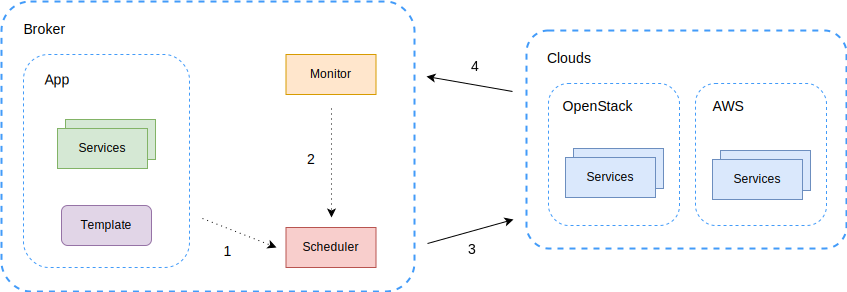
\includegraphics[width=\linewidth]{images/broker-cycle}
	\caption{Arbeitsweise des Multi-Cloud-Brokers als Zyklus: (1) Sammeln der Meta-Informationen alle Cloud-Provider, (2) Sammeln der Laufzeitinformationen der Anwendungen, (3) Sammeln der SLAs, (4) Nutzeränderungen: Neue Anwendungen oder Anpassung von SLAs, (5) Optimierungsplanung, (6) Planausführung auf den Cloud-Infrastrukturen}
	\label{fig:cycle}
\end{figure}

%Zyklus\autoref{fig:cycle}:

%\begin{description}
%	\item[Nummerierte Aufzählung]~\par
\begin{enumerate}
	
	\item Sammeln der Meta-Informationen alle Cloud-Provider
	\begin{enumerate}
		\item Kapazität (CPU, RAM, HDD, Network)
		\item Features (Verschlüsselung, CUDA, …)
		\item Geo-Lokation 
		\item Preis
	\end{enumerate}
	
	\item Sammeln der Laufzeitinformationen der PaaS/Anwendungen
	\begin{enumerate}
		\item Auslastung
		\item Fehler
		\item Ausfälle
	\end{enumerate}
	
	\item Sammeln der SLAs
	\begin{enumerate}
		\item Policy-Definitionen
		\item Policy-Konfiguration
		\item Placement-Algorithmen
	\end{enumerate}
	
	\item Neue Anwendung/Änderung eines SLA
	
	\item Optimierung
	\begin{enumerate}
		\item Feste Vorgaben (Geo, Backup)
		\item Weiche (Preis, Latenz, Verfügbarkeit)
	\end{enumerate}
	
	
	\item Ausführung
	\begin{enumerate}
		\item Netzwerkkonfiguration
		\item Allokation/De-Allokation von Ressourcen
		\item Deployment
		\item Migration
		\item Logging/Benachrichtigung
		\item Backup
	\end{enumerate}
	
\end{enumerate}

\section{Brokering}


%https://de.wikipedia.org/wiki/Constraintprogrammierung
%https://de.wikipedia.org/wiki/Scheduling

%entailing multiple constraint satisfaction (MCS)
%
%\todo{Schaubild, was wird wann gematcht}
%% Pseudocode des Algorithmus, wie in Meryn
%
%Kostenoptimierung
%
%Preisentwicklung? 
%
%Migration je nach Tageszeit? 
%
%Kosten der Datentransfers 
%
%Subscription On-Demand/Monthly/Yearly 
%
%Kompliziert durch undurchsichtige Staffelpreise
% https://www.rightscale.com/blog/cloud-cost-analysis/aws-vs-azure-vs-google-cloud-pricing-compute-instances

%https://www.rightscale.com/blog/cloud-cost-analysis/comparing-cloud-instance-pricing-aws-vs-azure-vs-google-vs-ibm

%
%Cost Calculators 
%
%http://go.appscale.com/cloud-cost-calculator-help 
%
%https://github.com/ifosch/accloudtant 
%
%https://awstcocalculator.com/# 
%

\section{Testumgebung: OpenStack \& Hyrise-R}

Hyrise\footnote{\url{https://hpi.de/plattner/projects/hyrise.html}} ist eine In-Memory-Forschungsdatenbank der Fachgruppe \emph{Enterprise Platform and Integration Concepts (EPIC)} am Hasso-Plattner-Institut \cite{grund:2010:hyrise}. Die Datenbank teilt sich einige Eigenschaften mit \emph{SAP HANA}\footnote{\url{https://www.sap.com/products/hana.html}}: Ein \emph{Delta Store}, spaltenorientierte Speicherung, Wörterbuchkodierung und weitere Komprimierungstechniken sowie den \emph{Insert-Only}-Ansatz und Partitionierung. Herausragend ist die OLAP-Performance, enthalten sind aber auch Optimierungen für OLTP-Aufgaben.

Hyrise-R ist eine Erweiterung des Basisprojektes um Replikation \cite{schwalb:2015:hyrise-r}. Es folgt dabei dem \emph{Scale-Out}-Ansatz: Alle schreibenden Operationen werden auf einem einzigen \emph{Master-Node} durchgeführt. Dessen Datensatz wird in weniger als einer Sekunde (\emph{lazy}) mit beliebig vielen \emph{Replica-Nodes} abgeglichen. Diese Spiegelungen bearbeiten alle reinen Leseanfragen und machen den Verbund so skalierbar, siehe \autoref{fig:hyrise-r}. Nach dem \emph{CAP-Theorem} sind Verfügbarkeit und Partitionstoleranz hier also wichtiger als Konsistenz. 

	\begin{figure}[ht]
	\centering
	\def\svgwidth{0.95\textwidth}
	\includesvg{images/hyrise-r}
	\caption{Verteilte \emph{Hyrise-R}-Architektur mit getrennter Verarbeitung von Lese- und Schreibanfragen. Der Master-Knoten dient als \emph{Single Source of Truth}. Zur Leistungssteigerung übernehmen Spiegelserver die Beantwortung der meisten Leseanfragen. Kleinere Inkonsistenzen werden dabei in Kauf genommen. Aus \cite{ssiclops:d42:experiments-measurements}.}	
	\label{fig:hyrise-r}
\end{figure}

Durch die verteilte Architektur ist Hyrise-R ein potenzieller Kandidat als Testanwendung innerhalb der Multi-Cloud-Umgebung. Einige \emph{SSICLOPS}-Teilprojekte untersuchten bereits Zuverlässigkeit, Performance, Datensicherheit und Vertraulichkeit in einer privaten OpenStack-Föderation \cite{ssiclops:d23:security-extensions, ssiclops:d42:experiments-measurements, bastian:2017:openstack-policies}. \todo{Diagramm:Hyrise-R on SSICLOPS}

Im Rahmen dieser Arbeiten sind einige Infrastrukturteile als Code veröffentlicht: So existiert zum Beispiel eine Docker-Teststellung mit grafischem Cluster-Manager, um die Performance bei verschiedenen Replikationsstufen zu prüfen. Diese Infrastruktur wurde in mehreren Studienarbeiten weiter angepasst, um Hyrise-R-KVM-Images in OpenStack bereitzustellen \cite{eschrig:2016:ssiclops-masterproject, maschler:2017:ssiclops-masterproject}. Möglicherweise können Teile dieser Arbeiten weiterentwickelt werden.


\section{Private-Cloud: OpenStack-Testbed}

Als Beispiel für eine Private-Cloud -- als Teil unseres Multi-Cloud-Setups -- soll OpenStack dienen. Es ist das populärste Open-Source-Projekt um eigene Infrastruktur als Service aufzubauen. Gesponsert wird es von Großunternehmen wie \emph{HPE}, \emph{IBM}, \emph{Canonical}, \emph{Red Hat} und anderen.

OpenStack setzt sich aus verschiedenen Teilprojekten zusammen, die jeweils einen Dienst entwickeln und bereitstellen. Ein Minimal-Setup besteht aus \emph{Nova} (Computing), \emph{Key\-stone} (Authentifizierung), \emph{Neutron} (Netzwerk) und \emph{Glance} (Images). Verbreitet sind außerdem \emph{Cinder} (Blockspeicher) und \emph{Horizon} (Dash\-board). Diese sollen auch in unserem Beispiel genutzt werden. Denkbar ist darüber hinaus die Integration eines Container-Dienstes. Der Zugriff auf die Infrastruktur erfolgt entweder über das Dashboard, Kommandozeilentools oder eine REST-API.

Grundsätzlich wäre auch der Aufbau einer OpenStack-Föderation wie in \emph{SSICLOPS} denkbar \cite{ssiclops:2015:d6.1-project-presentation}. Föderierte Cloud-Architekturen teilen sich zentrale Komponenten, in OpenStack mindestens den Authentifizierungsservice \emph{Keystone}. Je nach Föderationsvariante (\emph{Cells}, \emph{Regions}, \emph{Availability Zones} oder \emph{Host Aggregates}) sind auch Dienste wie Dashboard oder Speicher nur einmal vorhanden. Diese Architektur reduziert Fixkosten, erfordert allerdings spezielle Anpassungen innerhalb der Cloud. Auch gehen einige Vorteile wie Ausfallsicherheit und Unabhängigkeit der zentralen Dienste wieder verloren. Eine Kombination mit weiteren Cloud-Providern im Rahmen unseres Multi-Cloud-Setups ist denkbar, bleibt aufgrund der aufwendigen Einrichtung aber außen vor. Auch wäre der zusätzliche Erkenntnisgewinn vermutlich gering.\todo{SSICLOPS-OS-Architektur}

Selbst ein minimales OpenStack-Testsetup ist durch die diversen Dienste komplex. Denkbar wäre also auch die Nutzung von externen OpenStack-Angeboten. In diesem Projekt gibt es hierfür grundsätzlich drei mögliche Bereitstellungsmodelle: 

\begin{enumerate}
	\item Public Cloud
	\\\emph{Betrieb auf geteilter Cloud-Infrastruktur}
	
	\item Hosted Private Cloud
	\\\emph{Betrieb auf exklusiver Cloud-Infrastruktur}
	
	\item Lokale Testinstallation
	\\\emph{Betrieb auf eigener physischer oder virtueller Infrastruktur}
\end{enumerate}

\noindent Eine Liste öffentlicher OpenStack-Angebote findet sich auf der Projekthomepage\footnote{\url{https://www.openstack.org/marketplace/hosted-private-clouds/}}. Dort werden auch weitere Informationen wie Funktionsumfang und Zertifizierungen aufgeführt. 

Interessant ist zum Beispiel das Angebot der Deutschen Telekom \emph{Open Telekom Cloud\footnote{\url{https://cloud.telekom.de/en/infrastructure/open-telekom-cloud/}}}: eine Public Cloud auf OpenStack-Basis -- in Deutschland -- mit vollem Funktionsumfang und API-Zugriff. International bietet \emph{Rackspace} eine Hosted Private Cloud\footnote{\url{https://www.rackspace.com/openstack/}}. Beide eignen sich jedoch kaum, um kleine Experimente zu starten, sondern richten sich vor allem preislich an größere Organisationen und Unternehmen.

Kostenlos ist das Public-Cloud-Angebot \emph{TryStack}\footnote{\url{http://trystack.org/}}. Sponsoren wie \emph{Cisco}, \emph{NetApp}, \emph{Dell} und \emph{Red Hat} finanzieren das Projekt. Die Registrierung erfolgt über die Aufnahme in eine Facebook-Gruppe, anschließend soll hierüber auch der Zugang zur kostenlosen OpenStack-\emph{Liberty}-Instanz erfolgen. Während der gesamten Laufzeit dieser Arbeit war allerdings weder ein Login noch Kontakt zu den Organisatoren möglich.

Lokale OpenStack-Installationen sind aufwendig: Für jeden Dienst muss ein eigener physikalischer Rechner bereitstehen. Dementsprechend verweist die offizielle Dokumentation direkt auf die Vielzahl von OpenStack-Distributionen\footnote{\url{https://www.openstack.org/marketplace/distros/}}. Diese bieten fast immer einen vereinfachten Setup-Prozess und oft die Option statt physikalischen Rechnern virtuelle Maschinen oder Container zu nutzen. Wie auch bei den Hosted-Angeboten sind hier nicht alle Dienste verfügbar. In allen Paketen fehlt \emph{Zun}, der aktuelle Container-Service.

Speziell für lokale Test- und Entwicklungsumgebungen existiert \emph{DevStack}\footnote{\url{https://docs.openstack.org/devstack/latest/}}. Das offizielle OpenStack-Projekt installiert automatisiert die wichtigsten OpenStack-Dienste auf einer einzigen Maschine. Ausdrücklich unterstützt werden dabei auch VMs und \emph{LXC}-Container. Es soll daher als Erstes erprobt werden.

\section{DevStack virtualisiert inkl. Container-Support}

Während der Installation nimmt DevStack tief greifende Veränderungen am Hostsystem vor. Es müsste also auf einem separaten Server installiert werden. Dieser Abschnitt beschreibt den Versuch einer virtualisierten, reproduzierbaren DevStack-Testinstallation. Außerdem soll \emph{Zun} integriert werden. 

Ziel ist DevStack in einem Container auszuführen, genauso wie die darin gestarteten Compute-Nodes ebenso in einem -- nun verschachtelten -- Container bereitzustellen. Die Gründe hierfür sind zusammengefasst:

\begin{enumerate}
	\item Keine oder minimale Änderungen am Hostsystem
	\item Reproduzierbarer Testaufbau
	\item Schneller und rückstandsloser Reset
	\item Zustände (\emph{Snapshots}) speicherbar
	\item Schnelle Ausführung von Gastapplikationen
\end{enumerate}

\noindent Auch eine virtuelle Maschine löst die oben genannten Probleme. Theoretisch. Problematisch wird die Ausführungsgeschwindigkeit von Gastanwendungen in einem mit \emph{VirtualBox} virtualisierten OpenStack. Eine Lösung ist \emph{verschachteltes KVM}, das bereits in der Arbeit [1] erprobt wurde. Die Autoren empfehlen ihren Vorschlag bei bestehenden Erfahrungen mit \emph{libvirt}. Der damalige Versuchsaufbau stellt sich allerdings als instabil und nicht mehr reproduzierbar heraus.

\begin{figure}[ht]
	\centering
	\begin{subfigure}[b]{0.29\textwidth}
		\def\svgwidth{\linewidth}
		{\tiny
			\includesvg{images/devstack-bare-metal}}	
		\caption{Bare-Metal-Installation}
		\label{fig:sub:devstack-bare-metal}
	\end{subfigure}\hfill%
	\begin{subfigure}[b]{0.31\textwidth}
		\def\svgwidth{\linewidth}
		{\tiny
			\includesvg{images/devstack-vm}}	
		\caption{All-in-One-VM}
		\label{fig:sub:devstack-vm}
	\end{subfigure}\hfill%
	\begin{subfigure}[b]{0.31\textwidth}
		\def\svgwidth{\linewidth}
		{\tiny
			\includesvg{images/devstack-docker}}	
		\caption{DevStack in Docker}
		\label{fig:sub:devstack-docker}
	\end{subfigure}
	
	\caption{Verschiedene Installationsvarianten für eine OpenStack-Testinstallation mit DevStack auf einem einzelnen Host -- inklusive Unterstützung für Docker-Compute-Container und klassische VMs. Eine direkte Installation verändert unwiderruflich das gesamte Host-System \emph{(a)}. Eine VM benötigt mehr Ressourcen und kann die Geschwindigkeit der Gastanwendungen negativ beeinflussen \emph{(b)}. Die Installation in einem Container schafft Abstraktion und Reproduzierbarkeit ohne Geschwindigkeitskompromisse. Die Gastcontainer nutzen weiterhin den Kernel des Host-OS \emph{(c)}.}
	\label{fig:devstack}
\end{figure}

\emph{LXD}-Container könnten sich ebenfalls eignen. Im Gegensatz zu Docker führen sie mehrere Prozesse aus, erinnern also mehr an eine klassische virtuelle Maschine (ohne deren Overhead). Laut Entwickler \emph{Canonical} fokussiert sich \emph{LXD} speziell auf IaaS-Aufgaben\footnote{\url{https://www.ubuntu.com/containers/lxd}}. Ein LXD-DevStack-Setup birgt allerdings die gleichen Hürden\footnote{\url{https://docs.openstack.org/devstack/latest/guides/lxc.html}} wie ein Docker-Setup \cite{graber:2016:openstack-lxd}. Beachtenswert ist noch das OpenStack-Projekt \emph{Kolla}, das jeden OpenStack-Dienst in einem eigenen Docker-Container installiert\footnote{\url{https://cloudbase.it/openstack-kolla-hyper-v/}}.

Um Container innerhalb von OpenStack auszuführen, gibt es mehrere, teils konkurrierende Projekte. Alle lassen sich über Plugins in DevStack einbinden. Dies sind die wichtigsten \cite{singh:2017:containers-openstack}:

\begin{description}
	
	\item[Zun\footnotemark]\footnotetext{\url{https://wiki.openstack.org/wiki/Zun}} Eigenständige OpenStack-API zum Starten und Verwalten von diversen Containertypen, inklusive \emph{Docker}.
	
	\item[Nova Docker\footnotemark]\footnotetext{\url{https://wiki.openstack.org/wiki/Docker}} Im Gegensatz zu \emph{Zun} erfolgt die Docker-Containerverwaltung über die bekannte Nova-API. Das Projekt wurde eingestellt.
	
	\item[Nova LXD\footnotemark]\footnotetext{\url{https://linuxcontainers.org/lxd/getting-started-openstack/}} Parallel zu \emph{Nova Docker} erfolgt der Zugriff über die Nova-API. Das Projekt wird von \emph{Canonical} aktiv vorangetrieben. Weiterer Teil ist die Automatisierung via \emph{Juju}.
	
	\item[Magnum\footnotemark]\footnotetext{\url{https://wiki.openstack.org/wiki/Magnum}} Eine Self-Service-Lösung zur Orchestrierung auf Basis von \emph{Heat}. Stellt automatisiert Container Orchestration Engines (COEs) wie \emph{Docker Swarm} und \emph{Kubernetes} bereit.
	
\end{description}

\noindent DevStack in Docker wurde bereits vor einiger Zeit umgesetzt\footnote{\url{https://github.com/ewindisch/dockenstack}}. Da das Projekt nicht mehr gepflegt wird und auf das ebenfalls beendete \emph{Nova Docker} aufsetzt, erfolgt die Neuimplementierung mit folgenden Änderungen:

\begin{itemize}
	
	\item Ubuntu-LTS-Basis-Image 14.04 $\Rightarrow$ 17.10
	\item Mehrprozessunterstützung per \emph{systemd}\footnote{\url{https://docs.openstack.org/devstack/latest/systemd.html}}
	\item OpenStack-Version Kilo $\Rightarrow$ Pike
	\item libvirt/QEMU-Instanzen
	\item Nova Docker $\Rightarrow$ Zun
	\item Container-angepasste DevStack-Konfiguration
	\item Vollständige Netzwerkkonfiguration
	
\end{itemize}

\todo{Architektur-Diagramm}

\noindent Größte Hürde ist die Limitierung auf einen Prozess innerhalb eines Standard-Docker-Containers. Neuere DevStack-Versionen setzen auf \. Daher muss dies über die Umgebungsvariable \emph{ENV container docker} bekannt gemacht werden. Anschließend lässt sich \emph{systemd} über zwei weitere Workarounds starten\footnote{\url{https://github.com/moby/moby/issues/27202}}\footnote{\url{https://github.com/moby/moby/issues/9212}}.

\emph{Docker Build} bereitet das Image mit allen externen DevStack-Abhängigkeiten vor. Notwendige Dienste wie \emph{RabbitMQ} und \emph{MySQL} werden bereits im Voraus installiert. Das Container-Image führt beim Start nur noch die allerletzten Schritte des Setups aus. Ganz vorweg nehmen lässt sich das Setup nicht, weil während des Builds keine erweiterten Rechte vorliegen.

Nach erfolgreichem Start reicht das Kommando \emph{make run}, um per Zun einen \emph{Cirros}-Basis-Container\footnote{\url{https://docs.docker.com/samples/library/cirros/}} zu starten. Der Stand der gesamten OpenStack-Installation lässt sich per \emph{docker commit} oder experimentell per \emph{Docker-Snapshots}\footnote{\url{https://criu.org/Docker}} sichern.

Anpassbar sind im Skript OpenStack-Services und -Versionen, da DevStack direkt aus den Quellen installiert wird. So ändern sich allerdings selbst die Abhängigkeiten der als stabil gekennzeichneten Versionen. Das Prinzip Infrastruktur als Code geht hier nicht immer auf -- DevStack ist nicht zuverlässig reproduzierbar. \autoref{fig:devstack} vergleicht die Installationsvarianten.

Als \emph{Proof-of-Concept} ist die Integration von Docker, DevStack und Zun bisher einmalig. Der Code ist daher auf GitHub\footnote{\url{https://github.com/janmattfeld/DockStack}} veröffentlicht und zeigt einige \emph{Best Practices} und \emph{Lessons Learned} in Bezug auf die genannten Projekte.

Letztendlich greifen wir auf eine lokale \emph{Mirantis}-OpenStack-Installation aus dem \emph{SSICLOPS}-Projekt zurück. Die Infrastruktur ist virtuell und wird durch \emph{Fuel}\footnote{\url{https://www.mirantis.com/software/openstack/}} zuverlässiger wieder aufgebaut. Die Zun-Container-Dienste sind nicht enthalten; dafür aber alle anderen Kernfunktionen und APIs.


\section{Multi-Cloud-Bibliotheken}
\label{sec:bibliotheken}
\todo{Kleines Architektur Diagramm}

Ziel ist die Implementierung eines externen Broker-Services oder die Aufwertung einer verteilten Anwendung für den automatischen Betrieb in mehreren Clouds. Da unabhängige Cloud-Provider keine einheitlichen APIs anbieten, stellt dieses Kapitel verschiedene Bibliotheken vor, um möglichst viel der zusätzlichen Komplexität zu verbergen.

Ohne weitere Bibliotheken müsste für jede zu berücksichtigende Cloud das jeweilige SDK eingebunden werden. Auch Namensgebung, Architektur und Prozesse unterscheiden sich von Anbieter zu Anbieter. \todo{Mention Standard Cloud API OASIS TOSCA}

Durch den Einsatz einer Drittbibliothek ergibt sich allerdings eine potenzielle Schwachstelle. Falls diese fehlerhaft ist oder gar nicht weiter entwickelt wird, gefährdet dies das ganze Projekt. Historie und Zukunftschancen spielen bei der Auswahl eine zentrale Rolle. Im Optimalfall abstrahiert die Bibliothek Änderungen der Provider-SDKs. Ob und wie groß die Arbeitserleichterung ausfällt, prüft der Praxisteil.

Im Folgenden untersuchen wir die Eignung der populärsten Bibliotheken. Wichtigste Komponente ist dabei das Computing-Modul. Wünschenswert wäre auch Container-Unterstützung, um Images anbieterunabhängig bereitzustellen. Gestartete Anwendungskomponenten erfordern für die erste Erreichbarkeit oft Zugriff auf die DNS-Einstellungen der Cloud. Optional ist die Unterstützung von \emph{Content Delivery Networks}, Speicher- und Backup-Diensten.

% https://tex.stackexchange.com/questions/341592/hyphenating-text-inside-tabularx
\begin{table*}\centering
	\begin{minipage}{\textwidth}
		\caption{Übersicht freier Multi-Cloud-Bibliotheken. Mit $*$ gekennzeichnete Eigenschaften sind experimentell. Aufgeführt sind nur die populärsten Cloud-Provider, die Bibliotheken können darüber hinaus weitere unterstützen. Ob eine Bibliothek weitere Informationen, wie aktuelle Preisinformationen und den Standort des Rechenzentrums abrufen kann, zeigt die Spalte \emph{Cost\,/\,Geo}.}
		\ra{1.3}
		\begin{tabularx}{\textwidth}{>{\centering}XXXr} \toprule
			Projekt & Cloud-Provider & Cloud-Services & Cost\,/\,Geo\\ \midrule
			Apache Libcloud (Python)\footnotemark & AWS, Azure, OpenStack, GCP, Docker & Compute, Container, DNS, Load Balancer, Storage, Backup & $x$\,/\,$x$\\
			Apache jclouds (Java)\footnotemark & AWS, Azure, Open\-Stack$*$, GCP, Docker & Compute, Container, Load Balancer$*$, Storage & $x$\,/\,$x$\\
			PkgCloud (Node.js)\footnotemark & AWS, Azure, OpenStack& Compute, Load Balancer, Storage$*$, DNS$*$ & --\,/\,--\\
			Libretto (Go)\footnotemark & AWS, Azure, OpenStack, GCP & Compute & --\,/\,--\\
			Fog (Ruby)\footnotemark & AWS, OpenStack, GCP & Compute, DNS, Storage & $x*$\,/\,--\\
			\bottomrule
		\end{tabularx}
		\label{tab:bibliotheken}
		\vspace{150pt}
		\footnotetext[1]{\url{https://libcloud.apache.org/}}
		\footnotetext[2]{\url{https://jclouds.apache.org/}}
		\footnotetext[3]{\url{https://github.com/pkgcloud/pkgcloud/}}
		\footnotetext[4]{\url{https://github.com/apcera/libretto/}}
		\footnotetext[5]{\url{http://fog.io/}}
	\end{minipage}  
\end{table*}

\autoref*{tab:bibliotheken} listet die untersuchten Bibliotheken mit unterstützten Cloud-Providern, Services und weiteren Features. Letzteres sind Zugriff auf Preisinformationen des Anbieters und Standortinformationen der Rechenzentren. Zusätzlich sollten die Projekte kontinuierlich weiterentwickelt werden, eine aktive Entwicklergemeinschaft besitzen und gut dokumentiert sein. Alle sind Open Source und unter einer freien Lizenz verfügbar.

\begin{description}
	
	\item[Apache jclouds] existiert schon seit 2009. Es unterstützt zumindest experimentell die wichtigsten Provider, aber nicht alle Services: DNS ist nicht vorhanden, Container-Unterstützung gibt es nur für Docker. Die Bibliothek ist gut getestet, dokumentiert, und mit zahlreichen Beispielen ausgestattet. Durch Java ist sie außerdem typsicher. 
	
	\emph{jclouds} ist außerdem Grundlage mehrerer Multi-Cloud-Projekte, z.\,B. von \emph{Apache brooklyn\footnote{\url{https://brooklyn.apache.org/}}}: Mithilfe von \emph{CAMP}-Plänen lassen sich Anwendungen über mehrere Clouds ausrollen.
	
	\item[Apache Libcloud] vereint viele Vorteile: Es unterstützt neben OpenStack, als Referenz für Private-Cloud-Installationen, alle großen und kleinen Cloud-Provider mit allen Kernservices. Besonders interessant ist der Container-Support für \emph{Docker}, \emph{Kubernetes}, \emph{Amazon ECS} und die \emph{Google Container Engine}. Entsprechend gepackte Anwendungen könnten in einer Vielzahl von Clouds ohne weitere Änderungen ausgeführt werden.
	
	\item[Fog] integriert die wichtigsten Anbieter und Services. Die Entwicklergemeinde rund um \emph{Fog} ist aktiv und die Bibliothek wird häufig eingesetzt. Besonders interessant sind die bereitgestellten Mocks, die Tests des neuen Services erleichtern sollen. Zumindest für OpenStack wird Metering unterstützt. Eine einheitliche Namensgebung der verschiedenen Cloud-Produkte existiert nicht.
	
	\item[Libretto] beschränkt sich ausdrücklich auf die Compute-Funktionalität mithilfe virtueller Maschinen. Das zugehörige Projekt ist aktiv, kommt aufgrund der fehlenden Funktionalität aber nicht infrage.
	
	\item[PkgCloud] ist die einzige bekannte \emph{Node.js}-Bibliothek. Funktionsumfang und einheitliche Namensgebung der Cloud-Services sind überzeugend; leider wird die Bibliothek seit dem Verkauf des federführenden Unternehmens nicht mehr aktiv gepflegt. Bereits eingereichte Pull Requests werden nicht bearbeitet. Damit scheidet \emph{PkgCloud} für das Projekt aus.
	
\end{description}

\noindent Vielversprechend war außerdem das \emph{Apache DeltaCloud}-Projekt: Aufbauend auf \emph{Ruby} stellt es nicht nur eine einheitliche API nach \emph{Cloud Infrastructure Management Interface}-Standard\footnote{\url{https://www.dmtf.org/standards/cloud}} für die Kernfunktionen der wichtigsten Cloud-Provider, sondern auch zusätzliche Client-Bibliotheken und Mock-Funktionen. Aufgrund des plötzlichen Rückzugs von \emph{Red Hat} erfolgt seit 2013 allerdings keine Weiterentwicklung mehr \cite{androu:2013:deltacloud-red-hat-end}. Dieses Beispiel zeigt die Wichtigkeit nicht-funktionaler Betrachtungen bei der Auswahl einer Bibliothek. Auch Apache-Top-Level-Projekte haben nicht unbedingt eine sichere, vorhersagbare Zukunft.

Darüber hinaus existieren spezialisierte Bibliotheken wie \emph{SimpleCloud}\footnote{\url{https://framework.zend.com/manual/1.11/de/zend.cloud.html}} auf \emph{PHP}-Basis, das allerdings eine feste Komponente im \emph{Zend Framework} ist. Auch gibt es neue Entwicklungen wie \emph{CloudBridge}\footnote{\url{https://github.com/gvlproject/cloudbridge}} auf \emph{Python}-Basis. Besonderheit hier: Die Abstraktionsschicht nutzt die nativen SDKs der Cloud-Provider. \emph{CloudBridge} ist leider noch in einem frühen Entwicklungsstadium und als experimentell gekennzeichnet.

\emph{Libcloud} fasst die verschiedenen Cloud-Angebote nicht nur in gemeinsamen Namensräumen zusammen, sondern normalisiert auch Leistungsklassen. Python erleichtert außerdem den Einstieg und fügt sich in viele \emph{Python}-basierte Systemautomatisierungen ein. Diese Multi-Cloud-Bibliothek wird also im weiteren Verlauf der Arbeit erprobt.

%https://brooklyn.apache.org/learnmore/theory.html
% Apache Brooklyn hat eine eigene YAML-Service-Description-Spezifikation, ähnlich zu CAMP, der Clou Application Management API. Die Integration von TOSCA ist geplant, und in einer anderen Arbeit bereit umgesetzt: 
%Trans-Cloud: CAMP/TOSCA-based Bidimensional Cross-Cloud
% Keine SLAs, sondern nur Trigger-Action-Policies.
% Nutzt intern jclouds zur Provider-Anbindung.


\section{Entwicklungsumgebung}

% Hyrise-R-OpenStack- und Docker-Images, wie ersxtellt?

%Bestehende verteilte Anwendungen für den EInsatz in der CLoud vorbereiten, STichwort CLoud Native.
%Ausgangslage? Git-Repository mit teilautmatisierten Shell-Skripten und Makefiles. Automatisierung der Build, Test und Produktions-Infrastruktur, Ubuntu 16.04 auf Bare-Metal, VM und (Docker)Container.
%Integrieren der bestehenden Tests in diese Umgebungen.
%Packen des Geamtpakets aus Ausführungsumgebung, Programm und (Test-)Daten. auch automatisiert. Die Konfiguration ist variabel. SIe wird schematisch in der App-Konfiguration vorgegeben und dann von der CMP während der initialen Bereitstellung oder späteren Re-Deployments angepasst und ausgeführt.

% Tatsächliche Broker Architektur
% Code-Eigenheiten
% Tests/KPIs/Validierung der Hypothese

\section{Softwarearchitektur}

%as in Grozev 42: Federated CLoud Management: There is a central repository of images. this is replicated to the specific iaas/caas providers on demand.
%
%Alle weiteren Managementprozesse sind für Clients transparent.


\section{Multi-Provider-Service-Schema}

% D2.1: Übersicht Policy-Sprachen: Performance und Speichergröße. Entgegengesetzte Interessen. Lesbarkeit über zweiteiliung: Einmal für Menschen, einmal auf Bit-ebene für Maschinen. SLA über Proxy

%D2.2: Policys auf allen Schichten

%Matthias Bastian: Policy in OpenStack.

...und SLAs.

Ziel: Portabilität.

Mensch-und maschinenlesbar

YAML als aktuellen Standard

%TOSCA komplex, aber vielversprechend. Hierauf aufbauen (eigenen YAML-Entwurf erwähnen) und Brokering hinzufügen. Hier muss festgelegt erden, welcher Service-Teil auf welchem Provider mit welchem Instanz-Typen bereitgestellt werden soll. Dies soll automatisiert anhand von SLA/Policy und Preis entschieden werden. Unterstützt TOSCA deklarative Service-Definitionen?
%
%
%TOSCA hat folgendes nur optional
%- YAML (als SimpleVersion)
%- Multi-Provider als Plugin (nicht gewartet)
%- 
\begin{listing}[ht]	
	\inputminted[]{yaml}{./src/provider.sample.yaml}
	\caption{Provider-Definition und Zugangsdaten. Der Broker liest alle eingetragenen Accounts automatisch ein und berücksichtigt sie bei der initialen Service-Bereitstellung sowie in Optimierungsläufen. Public-Clouds benötigen nur Zugangsdaten wie Benutzername und Passwort -- alle weiteren Informationen erfragt der Broker dynamisch zur Laufzeit vom Provider. In Private-Cloud-Umgebungen ist dies nicht immer möglich: Details zur Verfügbarkeit, geografische Lage und Kosten müssen manuell eingepflegt oder vom Monitoring festgestellt werden.}
	\label{listing:provider}
\end{listing}



Platzhalter werden mit Jinja während des Deployments gefüllt.

Ablage der Pläne als Dokumentation.

Broker durch Metainformationen (und Labels) der Instanzen theoretisch zustandslos -> Broker selbst ist nicht ausfallgefährdet.

Erklärung der Metainformationen (versionierbar), verschiedenen Parameter und Rollenbeschreibung.

Je Provider Angaben zu Image und Startkommando. Dies wird hier eingetragen, um vom Broker dynamisch mit aktuellen Variablen angepasst zu werden: IP, Port...

Abhängig vom Service Level: IaaS/CaaS. Auch PaaS ist so denkbar. (Angabe als Image, Interpretation durch den Broker)

Beispiel verlinken.
Kapitel: Legacy Services Hyrise

Image-Erstellung und Repository.

Eigene Befehle
- Cloud-Init (Standard)
- shell/bash (Docker)

Vordefinierte Policys z.B. zum Verhalten im Fehlerfall. Aber auch Zusatzinformationen: Wie ist die Zustandsprüfung auf Service-Ebene auszuführen. Wichtig für Monitoring der Verfügbarkeit (SLA).

Abhängigkeiten von Services und wie oft global vorhanden? Hier: global ein master, abhängig vom Dispatcher.

\begin{listing}[ht]	
	\inputminted[firstline=15]{yaml}{./src/hyrise-r.sample.yaml}
	\caption{Providerübergreifende Servicevorlage. Der Ausschnitt zeigt die Definition des zentralen \emph{Hyrise-R-Dispatcher}-Dienstes. Nicht zu sehen sind Metadaten und die übrigen Anwendungsbestandteile. Parameter werden zur Laufzeit vom Broker eingesetzt.}
	\label{listing:hyrise-r}
\end{listing}

Könnte auch zu einem konkreten CAMP-Plan umgewandelt werden. So wie TOSCAMP. Stattdessen nur ein Template Schema und Graph zur Laufzeit.
%https://brooklyn.apache.org/v/latest/blueprints/setting-locations.html


\section{Tests und Diskussion}

%Kosten: Rechenzeit und Bandbreite (außerhalb einer Cloud) also gegenläufiges Ziel zu Portabilität und Ausfallsicherheit, denn die geringsten Kosten fallen bei dem Betrieb in einer einzelnen Cloud eines Providers an.
%i) providers’ pricing models, (ii) application’s communication patterns and (iii) distribution of nodes over providers.
%https://www.google.de/url?sa=t&rct=j&q=&esrc=s&source=web&cd=1&ved=0ahUKEwju27vHs6DZAhUCWRQKHRv7BEcQFggrMAA&url=http%3A%2F%2Fwww.mikesmit.com%2Fwp-content%2Fpapercite-data%2Fpdf%2Fcloud2012.pdf&usg=AOvVaw3e6yhHYmhWBbIxtr7MqkuX

%verschiedene OpenStack-Versionen haben unterschiedliche Schnittstellen. Auch dies kann über die Middleware abgefangen werden. RefStack testet API, Rally testet performance und führt tempest-Tests aus.


Aufwand einer Multi-Cloud-Strategie

Umsetzung der Policys

Potential

Vorteile durch Multi-Cloud-Bibliotheken

Aufwand für ein Multi-Cloud-Testbed